\documentclass[final]{beamer}

\usepackage{xparse}      % << to create new commands
\usepackage{tikz}   % << diagrams
  \usetikzlibrary{arrows}
\usepackage{url}

\usepackage[scale=1]{beamerposter}
\usetheme{confposter}

\setbeamercolor{block title}{fg=ngreen,bg=white}
\setbeamercolor{block body}{fg=black,bg=white}
\setbeamercolor{block alerted title}{fg=white,bg=dblue!70}
\setbeamercolor{block alerted body}{fg=black,bg=dblue!10}

\newlength{\sepwid}
\newlength{\onecolwid}
\newlength{\twocolwid}
\newlength{\threecolwid}
% A0 paper
\setlength{\paperwidth}{48in}
\setlength{\paperheight}{36in}

\setlength{\sepwid}{0.024\paperwidth}
\setlength{\onecolwid}{0.22\paperwidth}
\setlength{\twocolwid}{0.464\paperwidth}
\setlength{\threecolwid}{0.708\paperwidth}
\setlength{\topmargin}{-0.5in}

\usepackage{graphicx}  % Required for including images
\usepackage{booktabs} % Top and bottom rules for tables

% fonts
\usepackage{fontspec} 
\usepackage{xunicode}
\usepackage{xltxtra}
\defaultfontfeatures{Mapping=tex-text}
\setromanfont[Ligatures={Common},Numbers={OldStyle},Variant=01]{Linux Libertine O}

\title{Development of a Numerical Framework for the Study of Solid Earth Tides}
\author{Mattia Penati, Edie Miglio and Simone Carriero}
\institute{Politecnico di Milano - Department of Mathematics - MOX}

% ======================================================== math
\usepackage{listings}
\usepackage[ruled]{algorithm2e}
\usepackage{mathtools} % << extends amsmath
\usepackage{amsfonts}  % << some extra fonts
\usepackage[
  bold-style=ISO,
]{unicode-math}
\usepackage{nicefrac}  % << to make nice fraction

\setmathfont{Latin Modern Math}
\setmathfont[range=\mathbb]{TeX Gyre Pagella Math}

\DeclareDocumentCommand\defeq{}{\mathrel{\mathop:}=}
\DeclareDocumentCommand\dual{m}{#1^*}
\DeclareDocumentCommand\adj{m}{#1^T}
\DeclareDocumentCommand\inv{m}{#1^{-1}}
\DeclareMathOperator*{\Kernel}{Ker}
\DeclareMathOperator*{\Range}{Im}

\DeclareMathOperator{\grad}{\nabla}
\AtBeginDocument{
  \let\div\relax
  \DeclareMathOperator{\div}{div}
}
\DeclareMathOperator{\dev}{dev}
\DeclareDocumentCommand\vec{m o o}{ %
  \mathbf{#1}\IfValueT{#2}{_{#2}}\IfValueT{#3}{^{#3}} %
}
\DeclareDocumentCommand\tensor{m}{#1}

\DeclareDocumentCommand\inner{m m o}{ %
  {\left( #1 , #2 \right)}\IfValueT{#3}{_{#3}} %
}
\DeclareDocumentCommand\norm{m o o}{ %
  {\left\|{#1}\right\|}\IfValueT{#2}{_{#2}}\IfValueT{#3}{^{#3}} %
}
\DeclareDocumentCommand\duality{m m o}{ %
  {\left\langle #1 , #2 \right\rangle}\IfValueT{#3}{_{\dual{#3} \times #3}}
}

\begin{document}

\addtobeamertemplate{block end}{}{\vspace*{2ex}}
\addtobeamertemplate{block alerted end}{}{\vspace*{2ex}}

\setlength{\belowcaptionskip}{2ex}
\setlength\belowdisplayshortskip{2ex}

\begin{frame}[t]

\begin{columns}[t]

\begin{column}{\onecolwid} % The first column

\begin{alertblock}{Objectives}
The aim of this work is the development of some numerical tools for the
investigation of the effects of the Moon and Sun attraction on the Earth. The
problem shows an intrinsic time dependency, given by both the dynamics in time
of the celestial bodies and by the Earth deformation model.
\end{alertblock}

\begin{block}{Introduction}
The effects of the gravitational field of other celestial bodies are evident on
the Earth's seas levels varying daily because of the Moon tide. Even if not
immediatly visible, tidal effects have been measured on continents; this
phenomenon is known as solid Earth tide, that is the deformation of the Earth's
crust due to the Moon and Sun tidal forces.

The solid Earth tides have been already studied from an analytical and
theoretical point of view~\cite{Carcaterra-Doglioni:tidal-ratchet}. A numerical
finite element approximation of the Moon tidal force has been proposed
in~\cite{Xing:fe-tidal}, based on a very simple model of the Earth. Aim of this
work is to construct a scalable software suite implementing a numerical solver
for the solid Earth tide with larger complexity.

This problem shows an intrinsic time dependency, given by the dynamics of the
celestial bodies and the Earth's deformation model. First the relative position
of the Earth, Moon and Sun in time are determined, then the Earth's deformation
is modeled.

The modeling of the Earth deformation can approached assuming the
planet to be an isotropic viscoelastic medium. The choice of the viscoelastic
rheological model leads us to the solution of a linear viscoelasticity problem.
A solver for this problem has been developed and validated. A massive MPI
parallelization has been implemented to speed up the computations. 
\end{block}

\begin{block}{Viscoelastic model with tidal forces}
The Earth has been modeled as a continuum body, with an isotropic viscoelastic
rheology. The conservation of linear momentum and the definition of the
pressure are given by the equations
\[
  \div\tensor{\sigma} + \vec{f} = 0
  \quad\text{and}\quad
  \div\vec{u} + \frac{d}{2\mu} \frac{1-2\nu}{1+\nu} p = 0;
\]
with the stress tensor given by the constitutive equation
\[
  \tensor{\sigma} = -p \tensor{I} +
  \int_0^t e^{-\frac{t-s}{\tau}} 2\mu \dev\grad_s\dot{\vec{u}}(s) \, ds,
\]
where $\mu$, $\nu$ and $\tau$ are the shear modulus, the Poisson ratio and
relaxation time, respectively. These quantities are not constrained to a
particular model of the Earth and this gives us the ability to approach
different scenarios with little effort.

The term $\vec{f}$ is the tidal force acting on the Earth exerted by the other
celestial bodies:
\[
  \vec{f}(\vec{x}, t)= -\rho G \left[
    \sum_i \frac{M_i}{\norm{\vec{r}[i]}[][3](t)} \left(
      \tensor{I} -
      3 \frac{\vec{r}[i](t) \otimes \vec{r}[i](t)}{\norm{\vec{r}[i](t)}[][2]}
    \right)
  \right] \vec{x}.
\]
Where $\rho$ and $G$ are the Earth density and the Cavendish gravitation
constant, respectively. The sum ranges over the considered celestial bodies
with mass $M_i$ and located at position $\vec{r}[i](t)$.
\end{block}

\end{column} % End of the first column


\begin{column}{\onecolwid} % Begin of the second column

\begin{block}{Simulation of the celestial mechanics}
This task requires the numerical simulation of the gravitational influence of
each body of the solar system to determine the configuration of Sun, Earth and
Moon.  Since we are dealing with a mechanical problem, it is natural to choose
a geometric integrator, then \emph{Galerkin variational
integrators}~\cite{Miglio-Parolini:variational-integrators} will be used.

These schemes has been implemented in a C suite, the validation of the solver
has been done comparing the results generated by the implemented software with
the ones provided by NASA JPL HORIZONS System.
\begin{figure}
  \small
  \begin{center}
    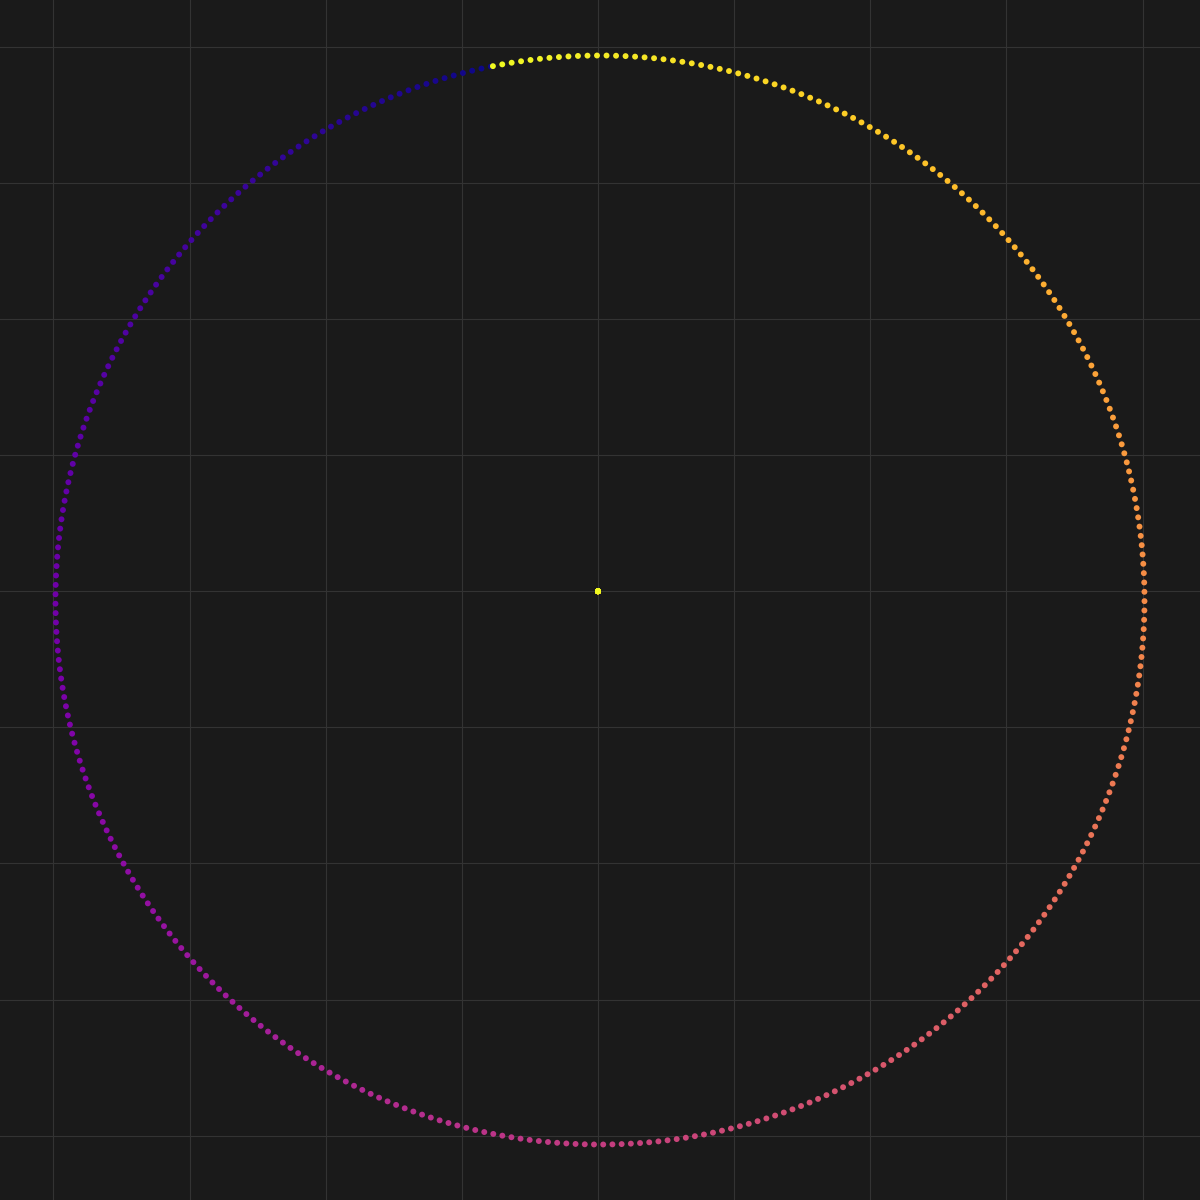
\includegraphics[width=0.37\textwidth]{images/three_bodies_sun_earth.png}
    \hspace{1em}
    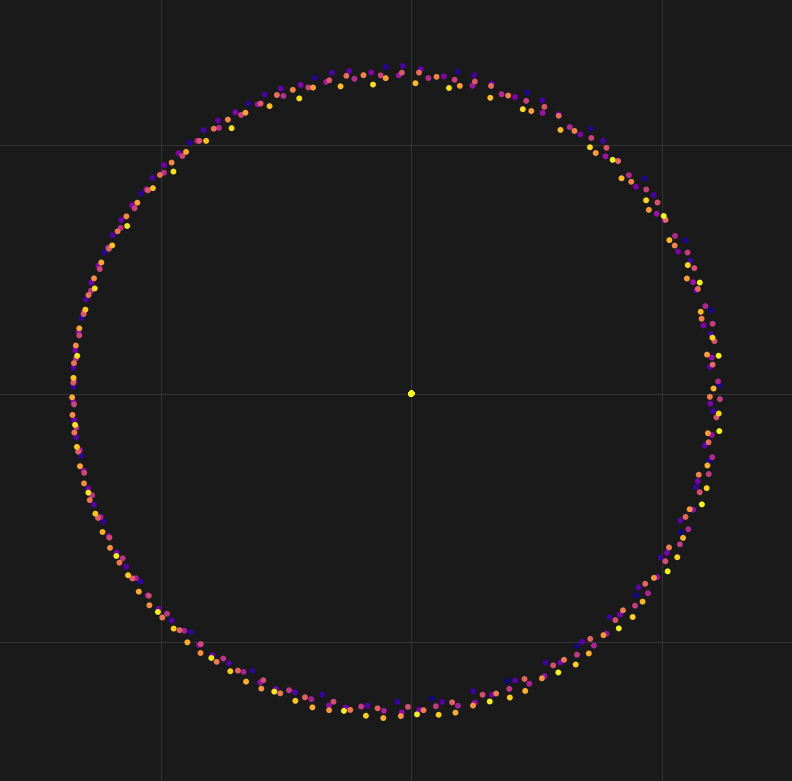
\includegraphics[width=0.37\textwidth]{images/three_bodies_earth_moon.png}
  \end{center}

  Simulated trajectories over 1 year long time range. On the \\
  left Sun-Earth trajectory and on the right Earth-Moon one.
\end{figure}
\end{block}

\begin{block}{Viscoelastic numerical solver}
A standard one-step, unconditionally stable and second-order accurate formula
based on mid-point quadrature is used to discretize the constitutive equation
with respect to time:
\[
  \begin{cases}
  \tensor{\sigma}_n = -p_n \tensor{I} +
    2 \mu e^{-\frac{\Delta t}{2\tau}} \dev \grad_s (\vec{u}[n]-\vec{u}[n-1]) +
    e^{-\frac{\Delta t}{\tau}} \tensor{h}_{n-1}, \\
    \tensor{h}_{n} = e^{-\frac{\Delta t}{\tau}} \tensor{h}_{n-1} +
      2 \mu e^{-\frac{\Delta t}{2\tau}} \dev \grad_s (\vec{u}[n]-\vec{u}[n-1]).
  \end{cases}
\]
A Discontinuous Galerkin scheme with Simmetric Weighted Interior Penalty
has been used to obtain a fully discretized problem, with the saddle point
structure
\[
  \begin{bmatrix}
    2 \hat{\mu} A & \adj{B} \\
    B & -\frac{d}{2\mu} \frac{1-2\nu}{1+\nu} M
  \end{bmatrix}
  \begin{bmatrix}\vec{u}[n] \\ p_n\end{bmatrix} =
  \begin{bmatrix}\vec{f}[n] \\ 0\end{bmatrix}
  \quad\text{with } \hat{\mu} = \mu e^{-\frac{\Delta t}{2\tau}}.
\]
If both the operators $\hat{A}\defeq A + \adj{B}\inv{M}B: V \to \dual{V}$ and
$M:Q \to \dual{Q}$ define an equivalent inner product on $V$ and $Q$, then all
the eigenvalues of the generalized problem
\[
  B\inv{\hat{A}}\adj{B}q = \lambda Mq, \qquad\text{in }\dual{Q},
\]
belong to the interval $[\beta^2,1]$. This result can be used to prove that the
following block operators
\[
  \begin{bmatrix}
    2\hat{\mu}A & \adj{B} \\
    B & -\frac{d}{2\mu} \frac{1-2\nu}{1+\nu} M
  \end{bmatrix}
  \qquad\text{and}\qquad
  \begin{bmatrix}
    2\hat{\mu} \hat{A} & -\adj{B} \\
    0 & \frac{d}{2\mu}M
  \end{bmatrix},
\]
are spectrally equivalent; the spectrum lies in $[-1, -\beta^2] \cup \{1\}$.
This defines an optimal block preconditioner for the problem.
\end{block}

\begin{block}{Implementation details}
The code is based on the finite element library deal.II \cite{dealII90},
version 9.0.0, which provided us with all the building blocks we needed. In
particular, a module in the library implements the geometric multigrid method
on hierarchical meshes with MPI support. This method has been used to implement
a preconditioner for the $\hat{A}$ block; the matrix $M$ is diagonal if a
proper pair of finite element space and quadrature rule is choosen. 
\end{block}

\end{column} % End of the second column


\begin{column}{\onecolwid} % The third column

\begin{block}{Results}
Two different problems have been built to measure the scaling
performance of the solver: one with a uniformly refined three dimensional
hyper-shell and one with a non-uniform grid.

\vspace*{.2em}
\begin{figure}
  \begin{center}
    \includegraphics[width=0.37\textwidth]{images/uniform_mesh.png}
    \hspace{1em}
    \includegraphics[width=0.37\textwidth]{images/linear_mesh.png}
  \end{center}
  \begin{center}
    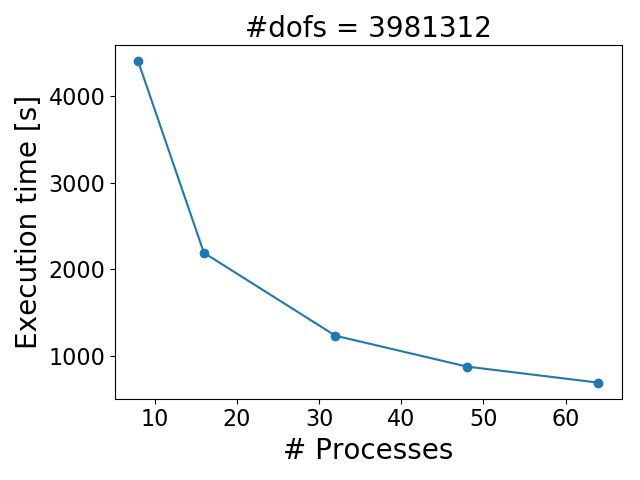
\includegraphics[width=0.37\textwidth]{images/uniform_scaling.png}
    \hspace{1em}
    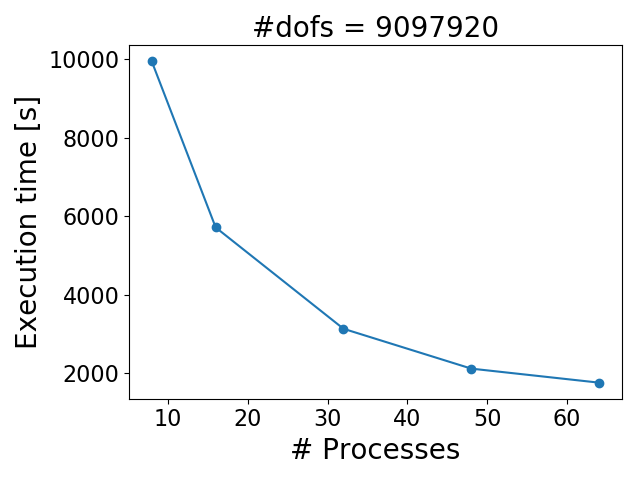
\includegraphics[width=0.37\textwidth]{images/linear_scaling.png}
  \end{center}
  \begin{center}
    \footnotesize
    \hspace{.5em}
    \begin{tabular}{ccc}
      \toprule
      \# procs & Elapsed time & Speed-up\\
      \midrule
      $8$  & $73$m $23$s & $-$   \\
      $16$ & $36$m $28$s & $2.01$\\
      $32$ & $20$m $31$s & $3.58$\\
      $48$ & $14$m $33$s & $5.04$\\
      $64$ & $11$m $28$s & $6.40$\\
      \bottomrule
    \end{tabular}
    \hspace{4.5em}
    \begin{tabular}{ccc}
      \toprule
      \# procs & Elapsed time & Speed-up\\
      \midrule
      $8$  &              $165$m $51$s & $-$   \\
      $16$ & \hspace{0.5em}$95$m $13$s & $1.74$\\
      $32$ & \hspace{0.5em}$52$m $07$s & $3.18$\\
      $48$ & \hspace{0.5em}$35$m $11$s & $4.71$\\
      $64$ & \hspace{0.5em}$29$m $12$s & $5.68$\\
      \bottomrule
    \end{tabular}
  \end{center}
\end{figure}
\vspace*{.2em}

We evaluate the solid tide effects on a time span of 28 days with constant
$\Delta t = 1$ hour. Two different configurations are shown: the first where
the Moon and Sun are almost aligned with the Earth; the second where the Moon
and the Sun form an angle of $\simeq90\text{°}$ with respect to the Earth. The
obtained results are of the same order of magnitude of the available
measurements.

\vspace*{.4em}
\begin{figure}
  \begin{center}
    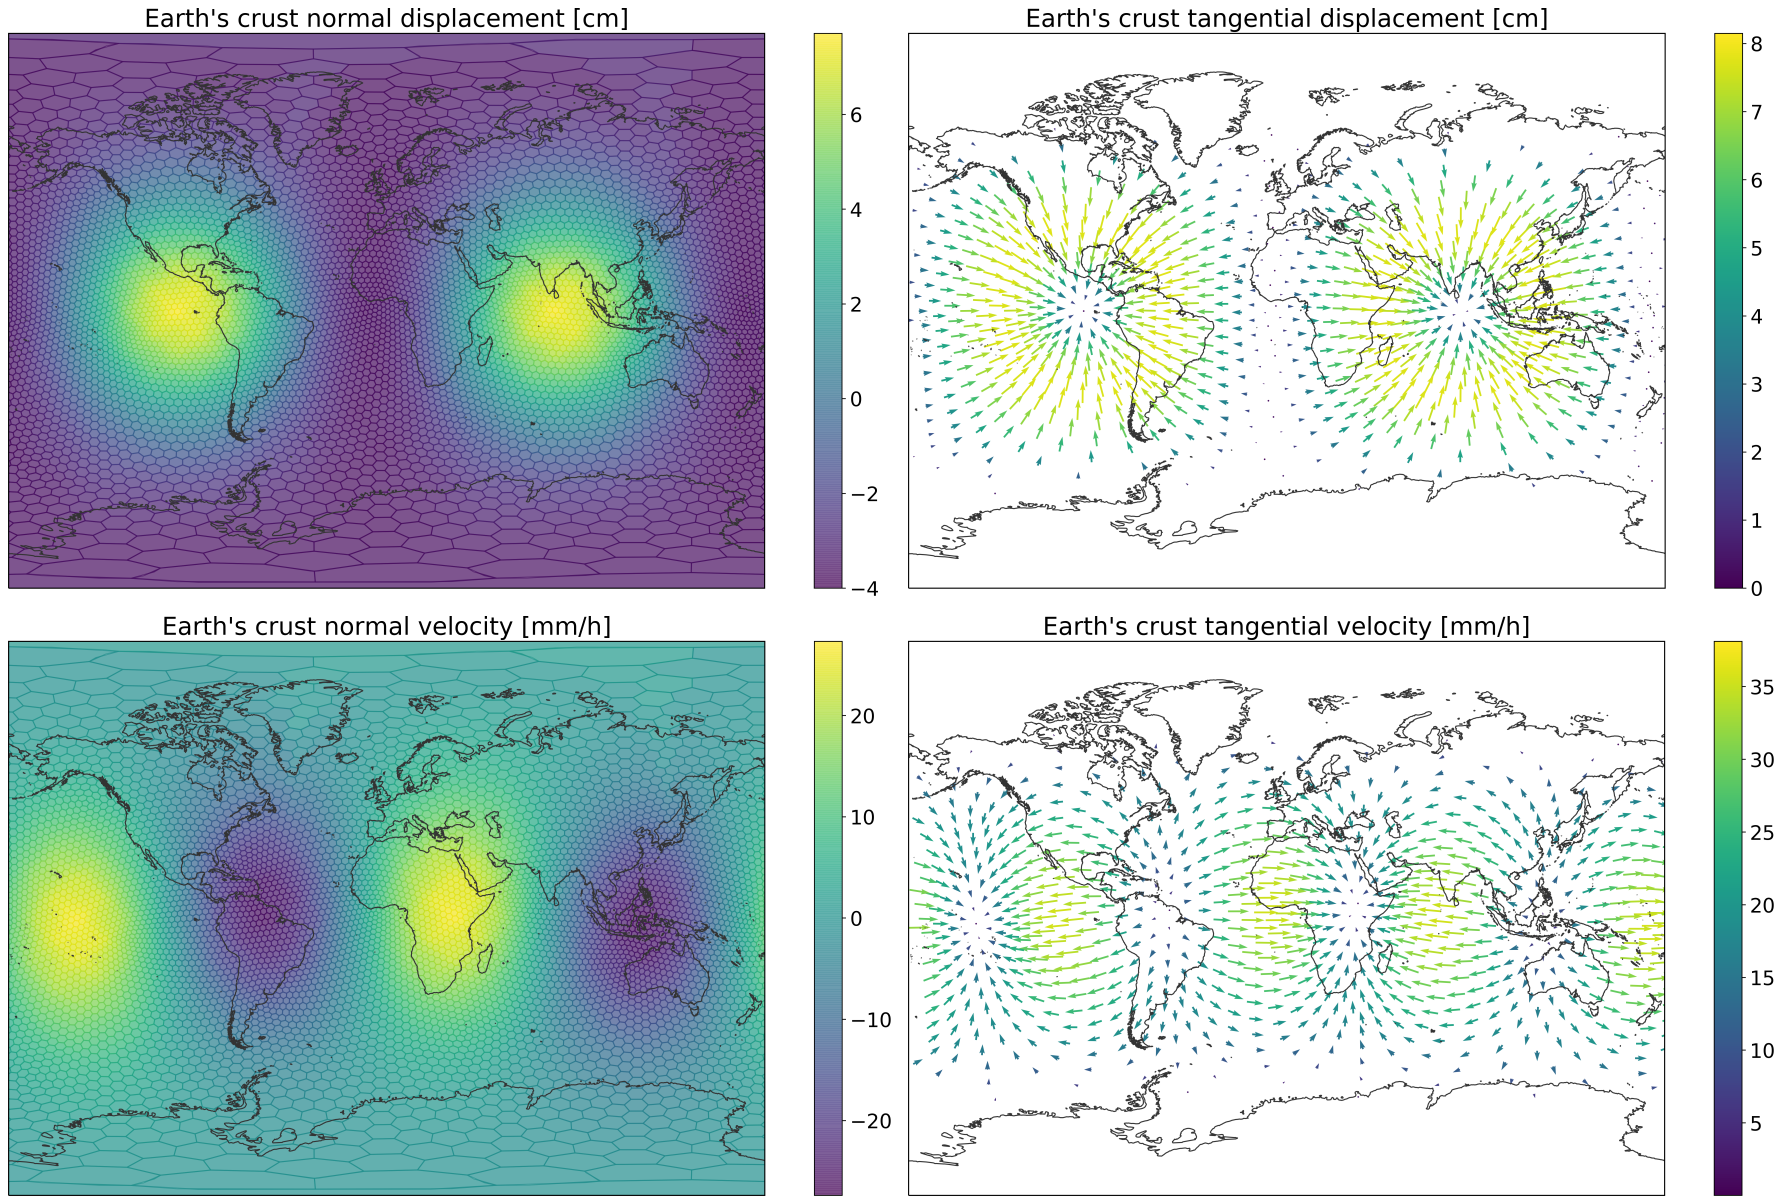
\includegraphics[width=0.94\textwidth]{images/viscoelastic001.png}
  \end{center}
\end{figure}
\vspace*{.4em}
\begin{figure}
  \begin{center}
    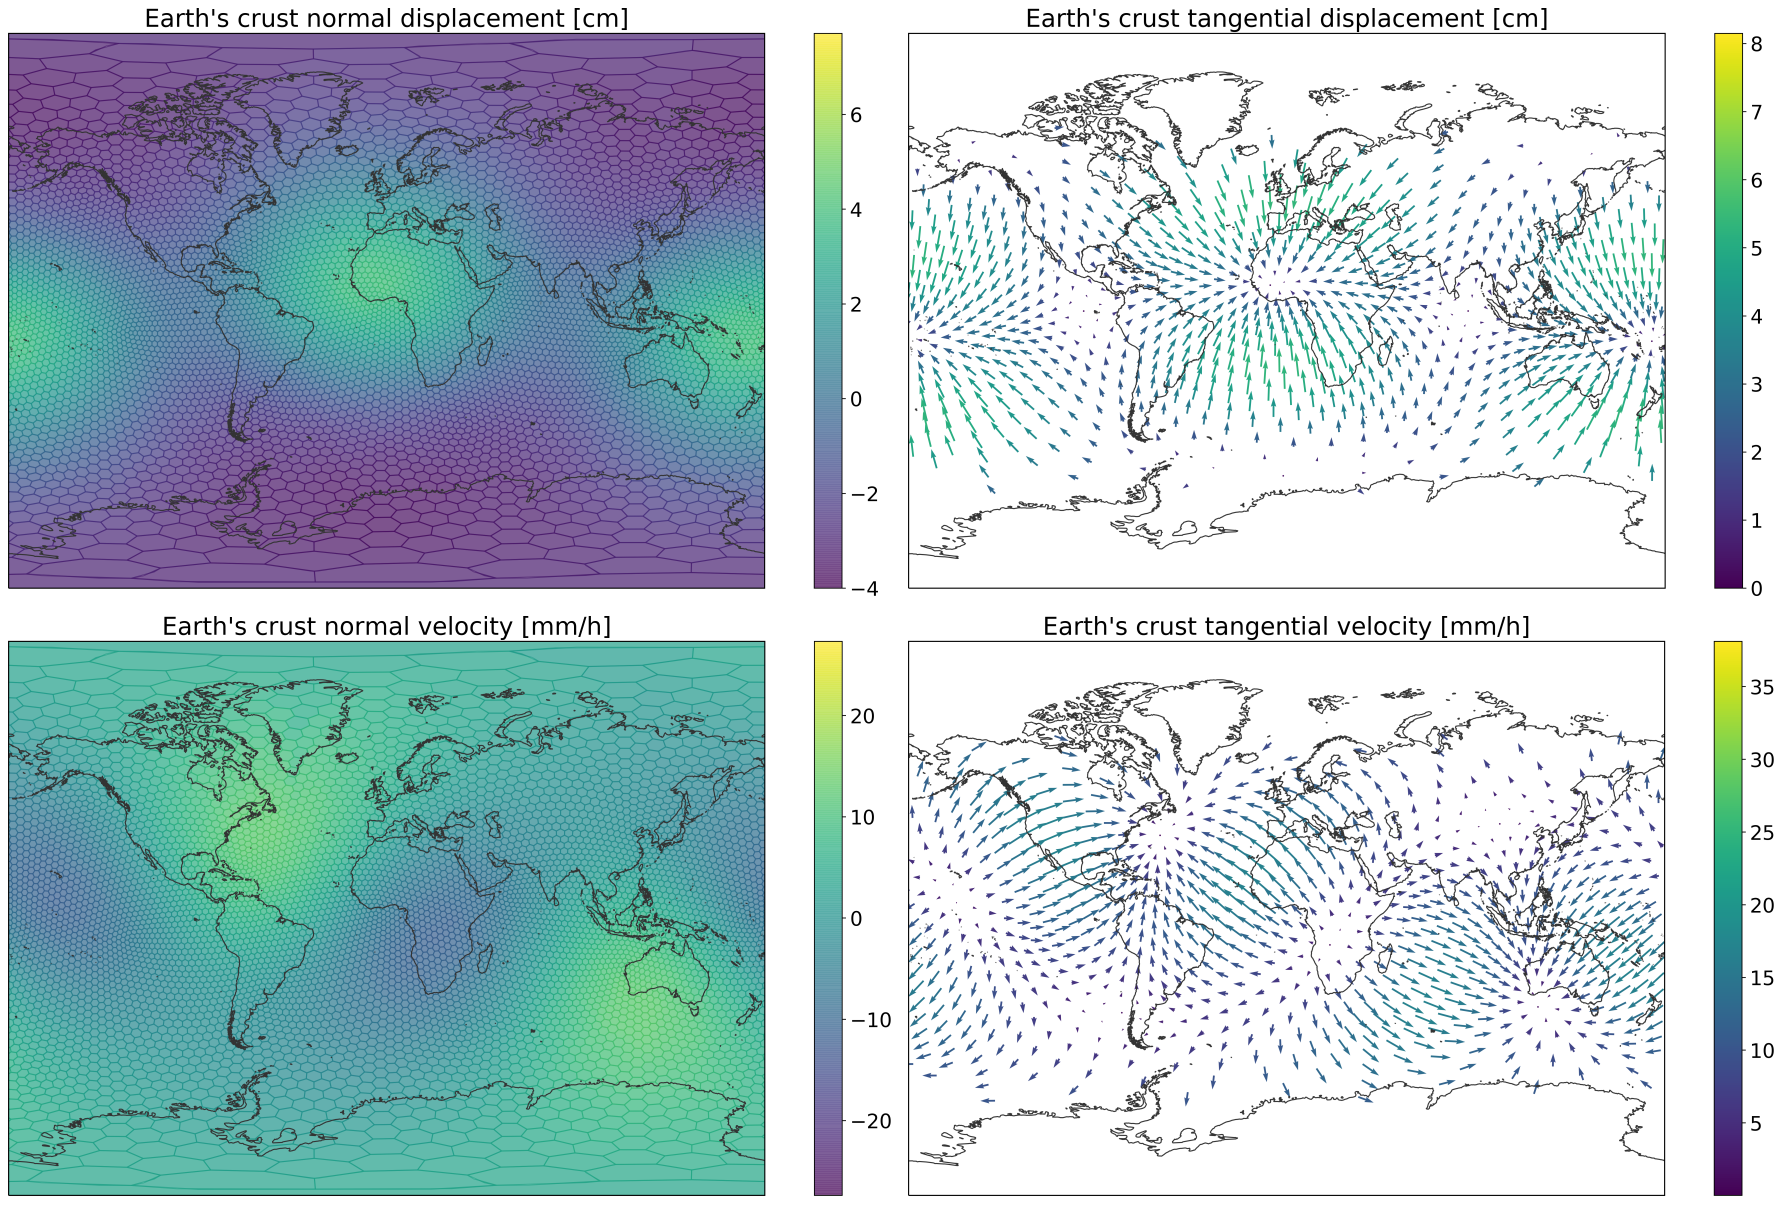
\includegraphics[width=0.94\textwidth]{images/viscoelastic169.png}
  \end{center}
\end{figure}
\end{block}

\end{column} % End of third column


\begin{column}{\onecolwid} % The fourth column

\begin{block}{Conclusions}
Solvers for these generic problems have been constructed, coded in a parallel,
scalable framework and strongly tested and validated.

The correctness of the convergence rate both in space and time of the adopted
numerical methods has been verified; moreover the optimality of the Geometric
Multigrid procedure adopted to precondition the algebraic version of the
problem has been confirmed.

The obtained results for the solid tides are exactly in the range of the
available measurements on the phenomenon and the ratio between the computed
lunar and solar tides is the expected one. The developed tool results to be
robust and is able to provide quantitative results in the constructed
scenarios.
\end{block}

\begin{block}{Future developments}
The first important enhancement required for the code is having a multiscale
time advancing method. This improvement will allow us to approach simulation on
wide time ranges, on which we expect viscous effects to be more relevant.

At the current stage the effects on the crust are visibile only if a proper
level of mesh refinement is reached. In order to reduce the number of the
unknowns a shell model can be used to obtain a more accurate description of the
Earth.
\end{block}

\begin{block}{References}

\nocite{*}
\footnotesize{\bibliographystyle{unsrt}
\bibliography{poster}\vspace{0.75in}}

\end{block}

\setbeamercolor{block alerted title}{fg=black,bg=norange}
\setbeamercolor{block alerted body}{fg=black,bg=white}
\begin{alertblock}{Contact Information}

\begin{itemize}
    \item Mattia Penati: \href{mailto:mattia.penati@polimi.it}{mattia.penati@polimi.it}
    \item Edie Miglio: \href{mailto:edie.miglio@polimi.it}{edie.miglio@polimi.it}
    \item Simone Carriero: \href{mailto:simone.carriero92@gmail.com}{simone.carriero92@gmail.com}
\end{itemize}
\begin{center}
    \begin{tabular}{ccc}
        
\includegraphics[width=0.4\linewidth]{images/logopoli} %
        & \hfill & %
        
\includegraphics[width=0.4\linewidth]{images/logomox}
    \end{tabular}
\end{center}
\hrulefill
\begin{columns}[onlytextwidth]
\begin{column}{0.83\textwidth}
    The poster can be downloaded from
    \begin{center}
        \footnotesize
        \url{https://bitbucket.org/mattiapenati/siamgs19-poster}
    \end{center}
\end{column}
\begin{column}{0.17\textwidth}
    
\includegraphics[width=0.99\textwidth]{images/qr}
\end{column}
\end{columns}

\end{alertblock}

\end{column} % End of the third column

\end{columns} % End of all the columns in the poster

\end{frame} % End of the enclosing frame

\end{document}
